\section{Privacy and Echo chambers}
To help visualize all the gathered data, to see the presence of echo chambers and to infer political views of users, data regarding followers of super-users has been used to create a social network graph and a cosine similarity matrix.

\subsection{Data Preparation}
First of all a list of super-users's followers has been gathered via TikTok APIs in the form of a JSON file, with the following structure (we can ignore \verb+"videoID"+ and \verb+"videoDate"+):

\begin{lstlisting}[language=json]
[
    {
        "influencer": "ith-super-user Name",
        "videoID": "videoID",
        "videoDate": "videoDate",
        "followerList": [
            "follower1",
            "follower2",
            "follower3",
            "follower4",
            "follower5",
            "follower6",
            "follower-k"
        ]
    }
]
\end{lstlisting}

For better understanding here follows a portion of the real JSON data used:

\begin{lstlisting}[language=json]
    {
        "influencer": "huffpost",
        "videoID": "7354208741996186911",
        "videoDate": "2024-04-05 11:46:08",
        "followerList": [
            "mathieucambet",
            "raphclp",
            "jennet153"
        ]
    },
    {
        "influencer": "huffpost",
        "videoID": "7354208741996186911",
        "videoDate": "2024-04-05 20:46:08",
        "followerList": [
            "doodlegolden0",
            "evanroyalaug",
            "cshanebritt",
            "kabed70"
        ]
    },
\end{lstlisting}

JSON data then gets imported to \textit{Social\_Graph.r} to analyze:

\begin{lstlisting}[language=R]
data <- fromJSON(paste(readLines("data.json")))

left_influencer_names <-  # vector of strings with left 
                          # super-user names
right_influencer_names <- # vector of strings with right 
                          # super-user names

# data.frame used to calculate all the graphs and tables
full_total <- data.frame(
  influencer = data$influencer,
  followerList = I(data$followerList)
)

full_influencer_names <- union(left_influencer_names, 
                               right_influencer_names)
\end{lstlisting}

Now we have three data structures to work with: two vectors with all super-user's names and a \verb+data.frame+ that stores all super-users and their gathered followers, like so: 

\aCapo{}
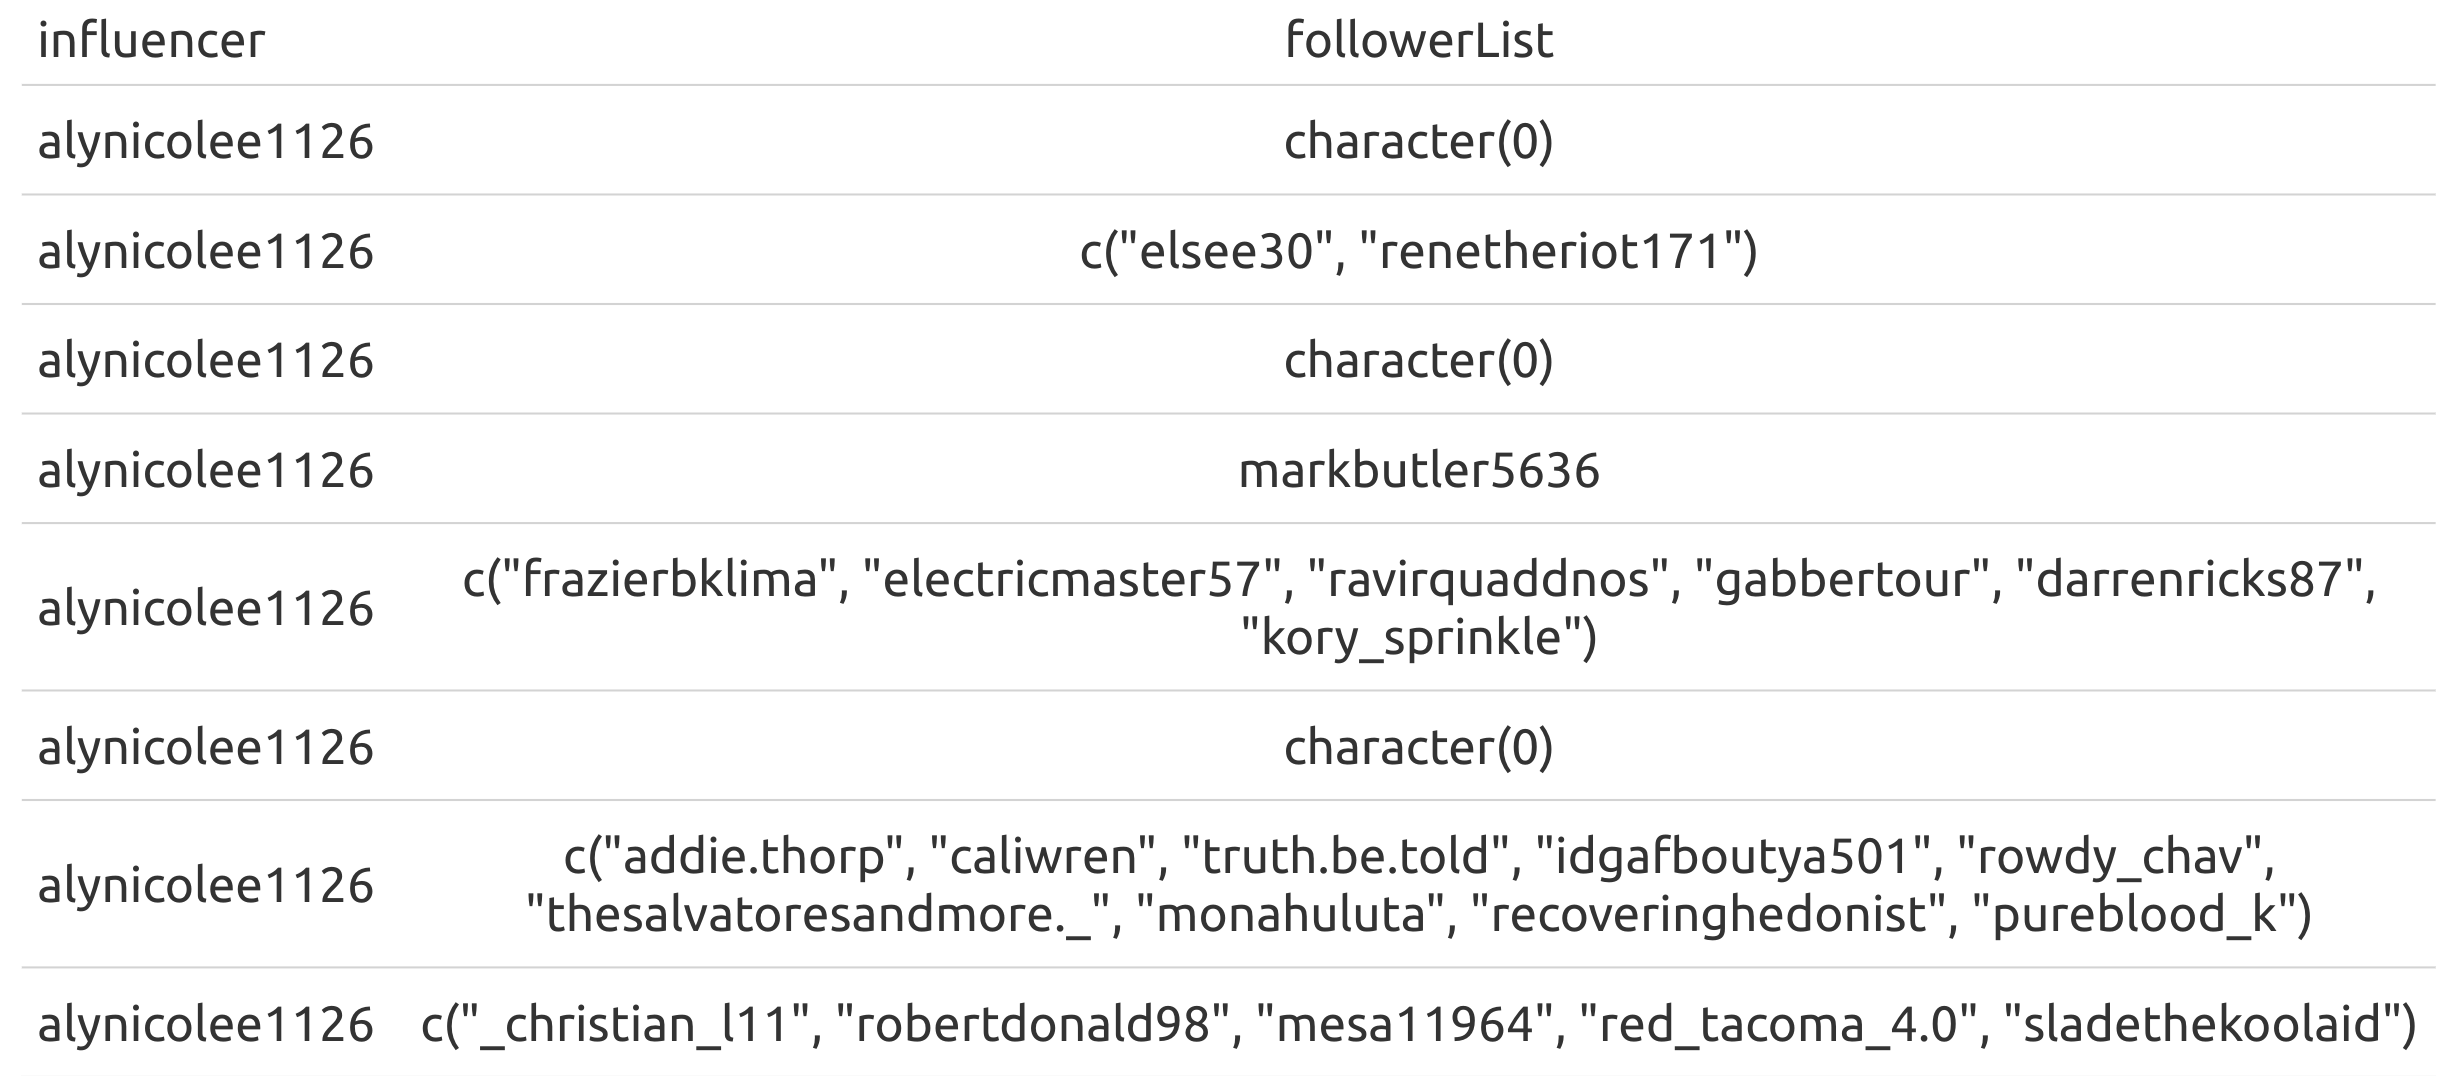
\includegraphics[width = .48\textwidth]{images/total_table_p23.png}

\subsection{Social Graph}
Broadly speaking, a social graph is a graph that represents social relations between entities, were vertices (or nodes) represents users and edges represents relations between such users. It is a model of representation of a social network, and has been referred to as "the global mapping of everybody and how they're related".\\ 
To give a brief example: if Alice and Bob are friends on a social network, in a social graph they would be represented each as a node, and there would be an edge between them.\\
The term was popularized at the Facebook F8 conference on May 24, 2007, when it was used to explain how the newly introduced Facebook Platform would take advantage of the relationships between individuals to offer a richer online experience \cite{wikiSAN}.

\aCapo{}
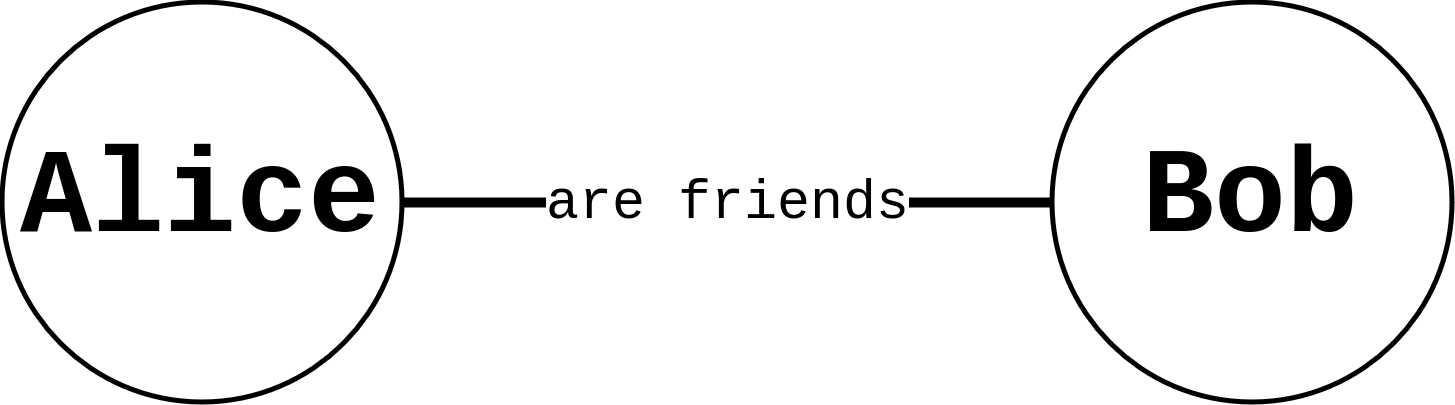
\includegraphics[width = .5\textwidth]{images/alice_bob_san.png}

Employing a social graph has numerous advantages: it helps visualize all gathered data (all users and their relations), visualize the presence of echo chambers and give insights to analyze the network as a whole. \\
The graph that follows clearly demonstrate that: considering the gathered data, users do not interact with each other outside their communities, thus forming cliques that can easily be interpreted as echo chambers:

\aCapo{}
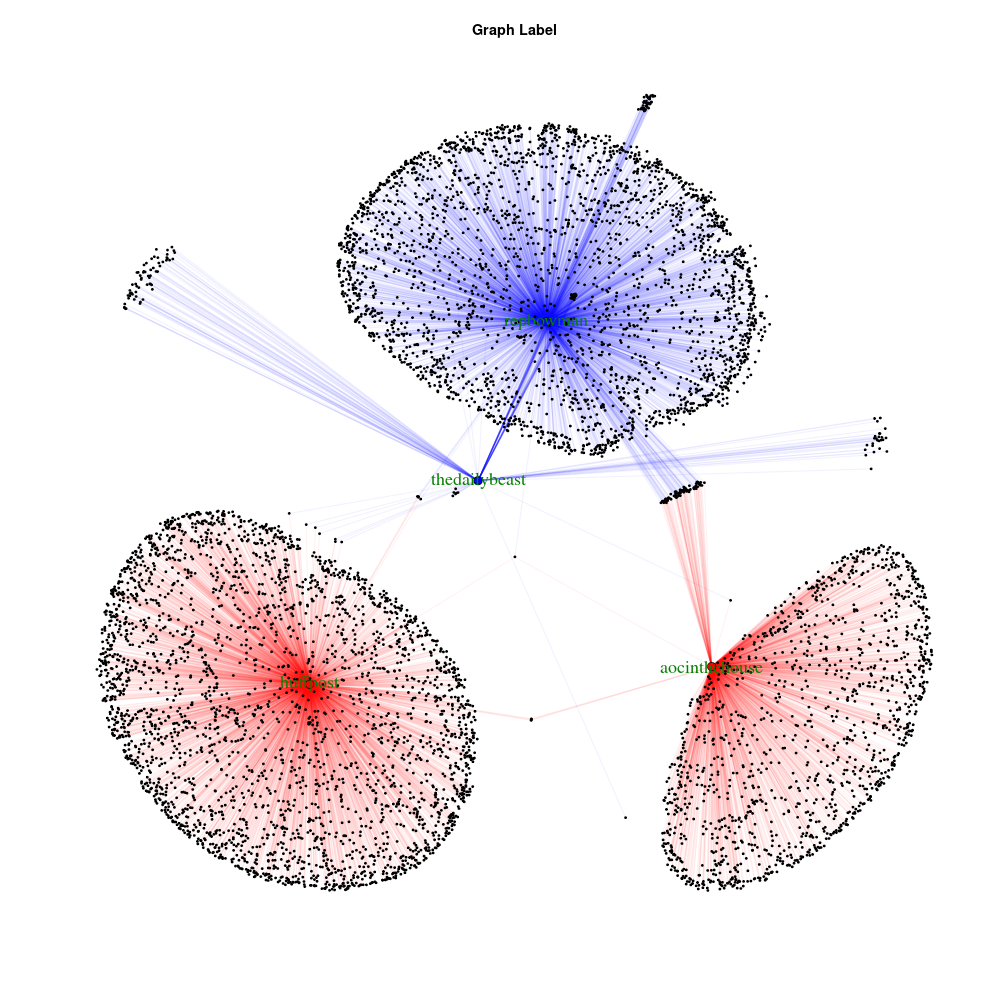
\includegraphics[width = .5\textwidth]{images/mockUP_san.png}

\textcolor{OrangeRed}{The aforementioned graph is actually a mockUp without all the complete data: due to hardware constraints, graph compilation is impossible at the moment of writing (04/06/2024).}\\
Super-users can be easily identified: their nodes are bigger than the rest, they are labeled and, most notably, the are at the center of their respective sub-graphs. \\
All black vertices represents followers of the super-users, unlabeled for improved readability, and the edge color represent the political orientation of the super-user to whom they are connected to(red for \textcolor{red}{right-leaning} and blue for \textcolor{blue}{left-leaning} super-users). \\
Lets clarify: if \textit{@user-Alice} follows super-user \textit{@aocinthehouse} (offical account of Congress member Alexandria Ocasio-Cortez), which is classified as a left-leaning super-user, the edge connecting them will be blue. \\
Conversely, if \textit{@user-Bob} follows super-user \textit{@thesun} (official account of UK's tabloid The Sun), which is classified as a right-leaning super-user, the edge connecting them will be red.

\subsection{Cosine Similarity}
Having a graphical representation of a network is certainly valuable: pictures are not only more effortless to recognize and process than words, but also easier to recall. When words enter long-term memory they do so with a single code. Pictures, on the other hand, contain two codes: one visual and the other verbal, each stored in different places in the brain (Paivio). The dual-coding nature of images allows for two independent ways of accessing visual memories, increasing the odds of remembering at least one of them. Adding illustrations to text, researchers have concluded, aids comprehension and learning \cite{10.21083/partnership.v10i1.3137}.\\
That being said, it is still advisable to measure numerically the similarity between users.\\
Broadly speaking, there are two types of similarity measures between nodes in a network: edge similarity, that provides the index of intersection of node parents (which are, of course among the neighbors) of the nodes being compared, and global structure similarity, that aims to evaluate the similarity between two nodes in the context of the whole network. Regarding the latter, Salton Index, Jaccard Index, and Sorensen Index always have good performance, while cosine similarity computational complexity is very high when applied to very large volumes of data \cite{smilarityMeasuresSurvey}: when the data is dense, the structure-based indices (like Salton's) can perform competitively good as Cosine index, while with lower computational complexity. Furthermore, when the data is sparse, the structure-based indices give even better results than Cosine index \cite{10.1016/j.phpro.2010.07.033}.\\

\aCapo{}
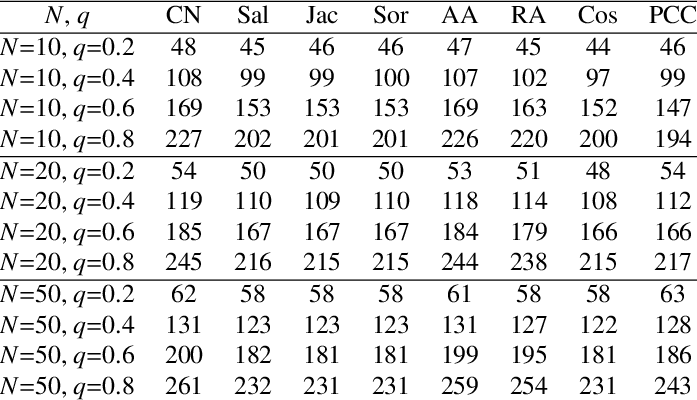
\includegraphics[width = .5\textwidth]{images/salton_precision.png}

The above table shows values regarding precision in inferring similarity between users: Salton index (\textit{Sal} column) seems to perform the best \cite{10.1016/j.phpro.2010.07.033}, therefore it has been used in this work to measure similarity between super-users.\\
Salton index formula is as follows: 

$$s_{xy}=\frac{|\Gamma(x)\cap\Gamma(y)|}{\sqrt{k_x\times k_y}}.$$

All index values are calculated for each couple of super-users, and are shown in the following table where, as mentioned before, blue represent left-leaning and red represent right-leaning super users: 

\aCapo{}
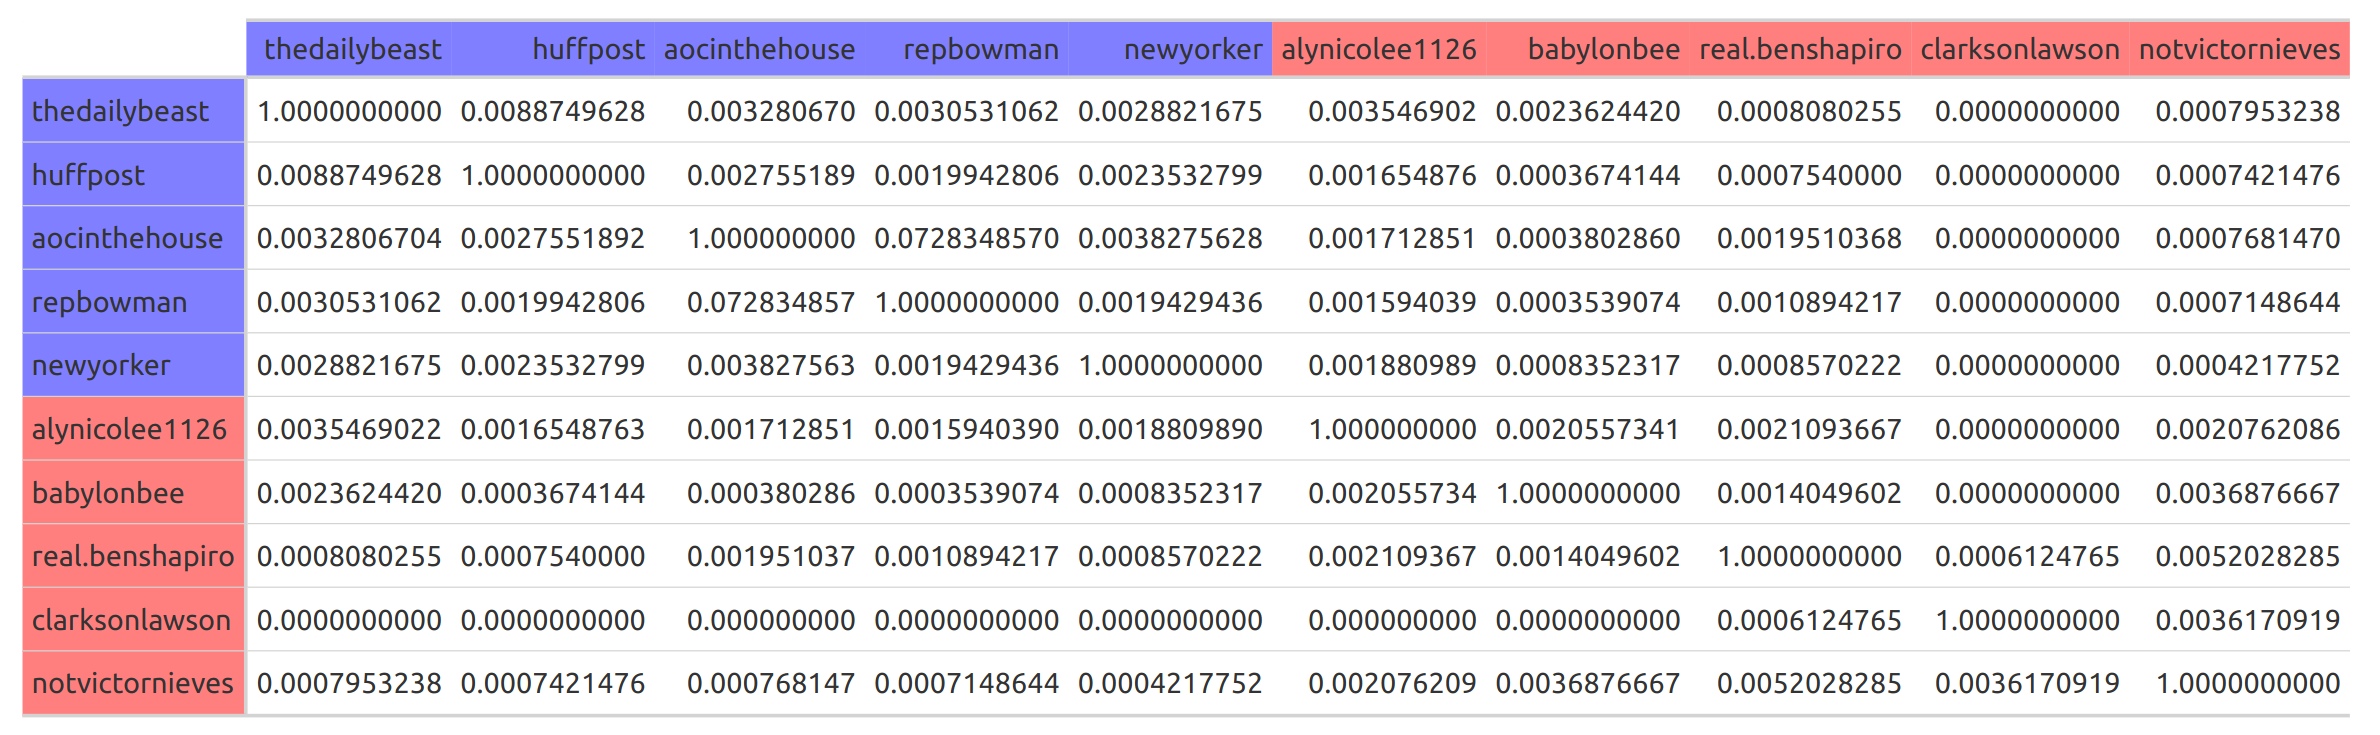
\includegraphics[width = .5\textwidth]{images/final_salton_matrix.png}

Salton index values range between 0 and 1, and the diagonal of the matrix represented in the table shows all values equal to 1 because, of course, a super-user is always identical to itself.\\
The table confirms numerically what could be seen in the social graph: super-users share very few followers, which means that each community is a form of echo chamber.

\subsection{Privacy Inference}